\documentclass[border=3pt]{standalone}
\usepackage{amsmath}
\usepackage{tikz}
\usetikzlibrary{positioning,fit,calc,arrows.meta,shapes.geometric,backgrounds}
\definecolor{nsGrey}{RGB}{210,210,210}
\definecolor{nsGreyD}{RGB}{110,110,110}
\definecolor{nsTeal}{RGB}{42,157,143}
\definecolor{nsTealD}{RGB}{31,111,101}
\definecolor{nsCoral}{RGB}{232,152,138}
\definecolor{nsPurple}{RGB}{142,124,195}
\definecolor{nsOrange}{RGB}{255,183,120}
\definecolor{nsPink}{RGB}{210,185,230}

\begin{document}
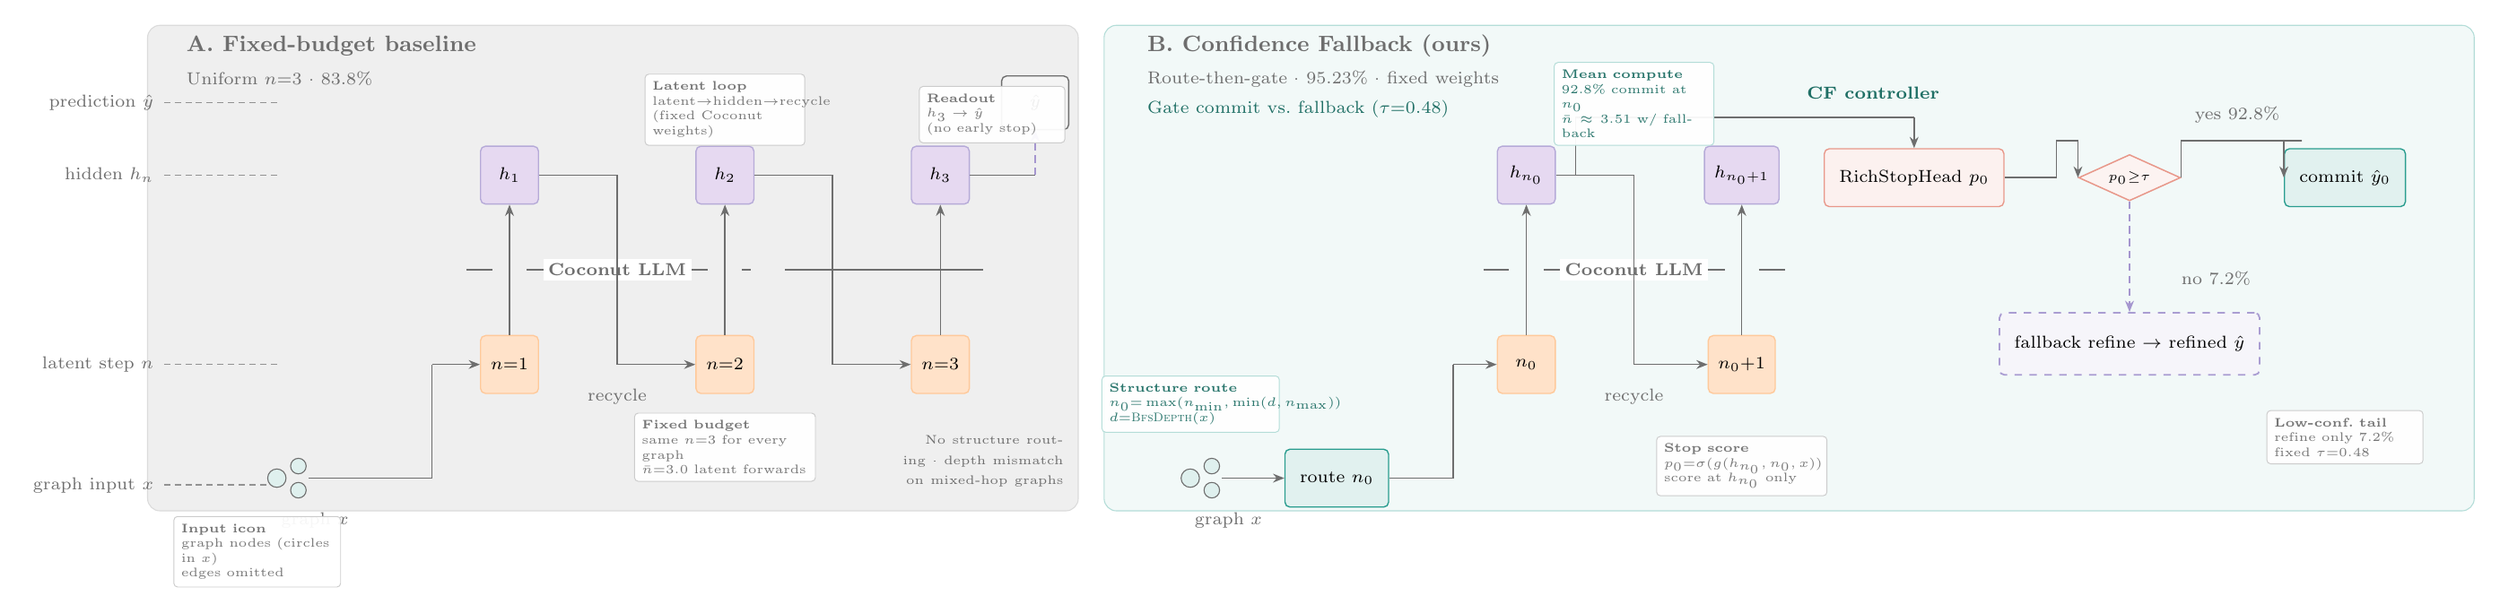
\begin{tikzpicture}[
  x=1.22cm, y=1.22cm,
  font=\small,
  hidden/.style={
    rectangle, draw=nsPurple!65, line width=0.5pt, fill=nsPink!55,
    rounded corners=2pt, minimum width=0.82cm, minimum height=0.82cm,
    inner sep=4pt, font=\scriptsize, align=center
  },
  embed/.style={
    rectangle, draw=nsOrange!75, line width=0.5pt, fill=nsOrange!40,
    rounded corners=2pt, minimum width=0.82cm, minimum height=0.82cm,
    inner sep=4pt, font=\scriptsize, align=center
  },
  bxteal/.style={
    rectangle, draw=nsTeal, line width=0.5pt, fill=nsTeal!14,
    rounded corners=2pt, inner sep=6pt, minimum height=0.82cm,
    font=\scriptsize, align=center
  },
  bxcoral/.style={
    rectangle, draw=nsCoral, line width=0.5pt, fill=nsCoral!14,
    rounded corners=2pt, inner sep=6pt, minimum height=0.82cm,
    font=\scriptsize, align=center
  },
  bxgrey/.style={
    rectangle, draw=nsGreyD, line width=0.5pt, fill=nsGrey!25,
    rounded corners=2pt, inner sep=6pt, minimum height=0.76cm,
    font=\scriptsize, align=center
  },
  gate/.style={
    diamond, draw=nsCoral, line width=0.55pt, fill=nsCoral!12,
    aspect=2.2, inner sep=2pt, minimum width=1.05cm,
    font=\tiny, align=center
  },
  fb/.style={
    rectangle, draw=nsPurple!75, line width=0.65pt, fill=nsPurple!8,
    rounded corners=2pt, inner sep=6pt, minimum height=0.88cm,
    font=\scriptsize, align=center, dashed
  },
  graphdot/.style={
    circle, draw=nsGreyD, fill=nsTeal!15, inner sep=0pt
  },
  ptitle/.style={font=\small\bfseries, text=nsGreyD},
  sub/.style={font=\scriptsize, text=nsGreyD},
  layerlbl/.style={font=\scriptsize, text=nsGreyD, align=right},
  wire/.style={line width=0.55pt, draw=nsGreyD},
  arrhd/.style={
    -{Stealth[length=1.6mm,width=1.25mm]},
    line width=0.55pt, draw=nsGreyD
  },
  darrhd/.style={
    -{Stealth[length=1.6mm,width=1.25mm]},
    line width=0.65pt, draw=nsPurple!80,
    dash pattern=on 3pt off 2pt
  },
  guidedash/.style={
    nsGreyD!75, line width=0.55pt, dash pattern=on 2.5pt off 1.8pt
  },
  ctrlbox/.style={
    draw=nsTeal!50, rounded corners=4pt, line width=0.55pt,
    inner sep=14pt, fill=nsTeal!4
  },
  note/.style={
    font=\tiny, text=nsGreyD, align=left,
    fill=white, fill opacity=0.94, draw=nsGreyD!35,
    rounded corners=1.5pt, inner sep=3pt, line width=0.35pt
  },
  notet/.style={
    font=\tiny, text=nsTealD, align=left,
    fill=white, fill opacity=0.94, draw=nsTeal!35,
    rounded corners=1.5pt, inner sep=3pt, line width=0.35pt
  },
]

% ---- spacious layer heights ----
\def\yP{1.02}
\def\yH{0.18}
\def\yM{-0.92}
\def\yE{-2.02}
\def\yG{-3.42}
\def\yBus{0.85}
\def\yGateBus{0.58}
\def\xAout{10.35}
\def\xScore{20.55}

% panel frames (wider / taller canvas)
\fill[nsGrey!35, rounded corners=5pt] (0.05,1.92) rectangle (10.85,-3.72);
\fill[nsTeal!6, rounded corners=5pt] (11.15,1.92) rectangle (27.05,-3.72);
\draw[nsGreyD!25, rounded corners=5pt] (0.05,1.92) rectangle (10.85,-3.72);
\draw[nsTeal!35, rounded corners=5pt] (11.15,1.92) rectangle (27.05,-3.72);

% ===================== Panel A =====================
\node[ptitle, anchor=west] at (0.40,1.68) {A.\ Fixed-budget baseline};
\node[sub, anchor=west] at (0.40,1.30) {Uniform $n{=}3$ · 83.8\%};

\node[layerlbl, anchor=east] at (0.22,\yP) {prediction $\hat y$};
\node[layerlbl, anchor=east] at (0.22,\yH) {hidden $h_n$};
\node[layerlbl, anchor=east] at (0.22,\yE) {latent step $n$};
\node[layerlbl, anchor=east] at (0.22,\yG) {graph input $x$};
\foreach \yy in {\yP,\yH,\yE,\yG} {
  \draw[guidedash] (0.24,\yy)--(1.55,\yy);
}

\node[graphdot, minimum size=2.6mm] (Ag0) at (1.55,\yG+0.08) {};
\node[graphdot, minimum size=2.2mm] (Ag1) at (1.80,\yG+0.22) {};
\node[graphdot, minimum size=2.2mm] (Ag2) at (1.80,\yG-0.06) {};
\coordinate (Agraphe) at (1.92,\yG+0.08);
\node[sub, anchor=north west] at (1.50,\yG-0.22) {graph $x$};

% three wide-spaced columns
\node[embed] (Ae1) at (4.25,\yE) {$n{=}1$};
\node[embed] (Ae2) at (6.75,\yE) {$n{=}2$};
\node[embed] (Ae3) at (9.25,\yE) {$n{=}3$};
\node[hidden] (Ah1) at (4.25,\yH) {$h_1$};
\node[hidden] (Ah2) at (6.75,\yH) {$h_2$};
\node[hidden] (Ah3) at (9.25,\yH) {$h_3$};
\node[bxgrey, minimum width=0.95cm] (Aout) at (10.35,\yP) {$\hat y$};

% Coconut LLM band — split line at column gutters; label off wire path
\draw[wire] (3.75,\yM) -- (4.05,\yM);
\draw[wire] (4.45,\yM) -- (5.35,\yM);
\draw[wire] (5.65,\yM) -- (6.55,\yM);
\draw[wire] (6.95,\yM) -- (7.05,\yM);
\draw[wire] (7.45,\yM) -- (9.75,\yM);
\node[font=\scriptsize\bfseries, text=nsGreyD, fill=white, inner sep=2pt, anchor=center]
  at (5.50,\yM) {Coconut LLM};

% wires (gutters between columns, never through boxes)
\draw[wire] (Agraphe) -- (3.35,\yG+0.08) -- (3.35,\yE);
\draw[arrhd] (3.35,\yE) -- (Ae1.west);
\draw[arrhd] (Ae1.north) -- (Ah1.south);
\draw[arrhd] (Ae2.north) -- (Ah2.south);
\draw[arrhd] (Ae3.north) -- (Ah3.south);
\draw[wire] (Ah1.east) -- (5.50,\yH) -- (5.50,\yE);
\draw[arrhd] (5.50,\yE) -- (Ae2.west);
\draw[wire] (Ah2.east) -- (8.00,\yH) -- (8.00,\yE);
\draw[arrhd] (8.00,\yE) -- (Ae3.west);
\node[sub, anchor=north] at (5.50,\yE-0.18) {recycle};

\node[sub, anchor=south east, align=right, text width=2.6cm] at (10.78,-3.54) {%
  \tiny No structure routing · depth mismatch on mixed-hop graphs%
};

% ===================== Panel B — latent lane =====================
\node[ptitle, anchor=west] at (11.55,1.68) {B.\ Confidence Fallback (ours)};
\node[sub, anchor=west] at (11.55,1.30) {Route-then-gate · 95.23\% · fixed weights};
\node[sub, anchor=west, text=nsTealD] at (11.55,0.95) {Gate commit vs.\ fallback ($\tau{=}0.48$)};

\node[graphdot, minimum size=2.6mm] (Bg0) at (12.15,\yG+0.08) {};
\node[graphdot, minimum size=2.2mm] (Bg1) at (12.40,\yG+0.22) {};
\node[graphdot, minimum size=2.2mm] (Bg2) at (12.40,\yG-0.06) {};
\coordinate (Bgraphe) at (12.52,\yG+0.08);
\node[sub, anchor=north west] at (12.10,\yG-0.22) {graph $x$};

\node[bxteal, minimum width=1.08cm] (Broute) at (13.85,\yG+0.08) {route $n_0$};
\node[embed] (Be0) at (16.05,\yE) {$n_0$};
\node[embed] (Be1) at (18.55,\yE) {$n_0{+}1$};
\node[hidden] (Bh0) at (16.05,\yH) {$h_{n_0}$};
\node[hidden] (Bh1) at (18.55,\yH) {$h_{n_0+1}$};

\draw[wire] (15.55,\yM) -- (15.85,\yM);
\draw[wire] (16.25,\yM) -- (17.15,\yM);
\draw[wire] (17.45,\yM) -- (18.35,\yM);
\draw[wire] (18.75,\yM) -- (19.05,\yM);
\node[font=\scriptsize\bfseries, text=nsGreyD, fill=white, inner sep=2pt, anchor=center]
  at (17.30,\yM) {Coconut LLM};

\draw[arrhd] (Bgraphe) -- (Broute.west);
\draw[wire] (Broute.east) -- (15.20,\yG+0.08) -- (15.20,\yE);
\draw[arrhd] (15.20,\yE) -- (Be0.west);
\draw[arrhd] (Be0.north) -- (Bh0.south);
\draw[arrhd] (Be1.north) -- (Bh1.south);
\draw[wire] (Bh0.east) -- (17.30,\yH) -- (17.30,\yE);
\draw[arrhd] (17.30,\yE) -- (Be1.west);
\node[sub, anchor=north] at (17.30,\yE-0.18) {recycle};

% ===================== Panel B — CF controller (wide internal spacing) =====================
\node[bxcoral, minimum width=1.15cm] (Bscore) at (20.55,0.15) {RichStopHead $p_0$};
\node[gate] (Bgate) at (23.05,0.15) {$p_0{\ge}\tau$};
\node[bxteal, minimum width=1.08cm] (Bout) at (25.55,0.15) {commit $\hat y_0$};
\node[fb, minimum width=2.35cm] (Bfallback) at (23.05,-1.78) {%
  fallback refine $\rightarrow$ refined $\hat y$%
};

\begin{scope}[on background layer]
  \node[ctrlbox, fit=(Bscore)(Bgate)(Bout)(Bfallback)] (Bctrlbox) {};
\end{scope}
\node[sub, anchor=south west, text=nsTealD] at ([xshift=4pt,yshift=2pt]Bctrlbox.north west)
  {\textbf{CF controller}};

\draw[arrhd] (Bscore.east) -- (22.20,0.15) -- (22.20,\yGateBus) -- (Bgate.west |- 0,\yGateBus) -- (Bgate.west);
\draw[arrhd] (Bgate.east) -- (Bgate.east |- 0,\yGateBus) -- (25.05,\yGateBus) -- (Bout.west |- 0,\yGateBus) -- (Bout.west);
\draw[darrhd] (Bgate.south) -- (Bfallback.north);
\node[sub, anchor=south] at (24.30,\yGateBus+0.10) {yes 92.8\%};
\node[sub, anchor=west] at (23.55,-1.02) {no 7.2\%};

% key arrows drawn last (on top): ŷ from below, RichStopHead from above
\draw[wire] (Ah3.east) -- (\xAout,\yH);
\draw[darrhd] (\xAout,\yH) -- (Aout.south);
\draw[wire] (Bh0.east) -- (16.62,\yH) -- (16.62,\yBus) -- (\xScore,\yBus);
\draw[arrhd] (\xScore,\yBus) -- (Bscore.north);

% full callouts — kept for density; placed in panel whitespace (after wires)
\node[note, anchor=north, text width=2.35cm] at (6.75,-2.58) {%
  \textbf{Fixed budget}\\same $n{=}3$ for every graph\\$\bar{n}{=}3.0$ latent forwards%
};
\node[note, anchor=south, text width=2.05cm] at (6.75,0.52) {%
  \textbf{Latent loop}\\latent$\to$hidden$\to$recycle\\(fixed Coconut weights)%
};
\node[note, anchor=north west, text width=2.15cm] at (0.35,-3.78) {%
  \textbf{Input icon}\\graph nodes (circles in $x$)\\edges omitted%
};
\node[note, anchor=south, text width=1.85cm] at (9.85,0.55) {%
  \textbf{Readout}\\$h_3\to\hat y$\\(no early stop)%
};

\node[notet, anchor=west, text width=2.30cm] at (11.12,-2.48) {%
  \textbf{Structure route}\\$n_0{=}\max(n_{\min},\min(d,n_{\max}))$\\$d{=}\textsc{BfsDepth}(x)$%
};
\node[notet, anchor=south, text width=2.05cm] at (17.30,0.52) {%
  \textbf{Mean compute}\\92.8\% commit at $n_0$\\$\bar{n}\approx 3.51$ w/ fallback%
};
\node[note, anchor=north, text width=2.20cm] at (18.55,-2.85) {%
  \textbf{Stop score}\\$p_0{=}\sigma(g(h_{n_0},n_0,x))$\\score at $h_{n_0}$ only%
};
\node[note, anchor=north, text width=2.00cm] at (25.55,-2.55) {%
  \textbf{Low-conf.\ tail}\\refine only 7.2\%\\fixed $\tau{=}0.48$%
};

\end{tikzpicture}
\end{document}
